\documentclass[a4paper,11pt]{article}
\usepackage{graphicx}

\textwidth15.5cm \textheight23cm
\oddsidemargin2mm \evensidemargin2mm \topmargin-10mm
\nonfrenchspacing
\parskip0.15\baselineskip

\title{The Technology of MUMIE-JAPS}
\author{Tilman Rassy $<$rassy@math.tu-berlin.de$>$\\ Ruedi Seiler $<$seiler@math.tu-berlin.de$>$}

\newcommand{\minorheadline}[1]{\textbf{#1:}}
\newcommand{\Mumie}{\textsc{Mumie}}

\begin{document}

\maketitle


\begin{center}
{\verb'$Id: techn_mumie_japs.tex,v 1.1 2008/04/14 10:31:12 rassy Exp $'}
\end{center}

\section{The Learning Environment MUMIE}

MUMIE is an e-learning platform optimized for experiencing, learning and
teaching mathematics in a multimedia environment going far beyond simple
document handling. Content in the form of fine granular, reusable and
interactive elements are organized in math-conform ontologies and can be
put and brought to action in different learning scenarios.  Visualisation
of scientific relations in the form of science nets makes possible
non-linear navigatin in the "Legoland of Mathematical Building Blocks".

MUMIE comprises several parts, one of which is JAPS, MUMIE's server-side
software. This paper is about JAPS. Other parts of MUMIE are the authoring
tools and the so-called Mathlet Factory. They are not covered by this paper.


\section{Design principles}

The design of the JAPS is based on the following principles:
\begin{itemize}
\item \minorheadline{Strict separation of content and presentation}
  Content contains no layout information and is completely independent of the context in
  which it is rendered.
\item \minorheadline{Dynamical creation of web pages}
  Almost any web material, including (X)HTML pages, CSS stylesheets, XSL stylesheets, and
  Java\-Script files, are created dynamically. This allows for a maximum of user
  adaptivity. To some extent, this is possible with binary contents as, for instance,
  pictures and applets, too, since JAPS can choose between different `realisations' for the
  same `generic' document depending on the context.
\item \minorheadline{XML technology}
  Non-binary content is stored as XML in the database. This is true not only for
  (X)HTML pages, but also for CSS stylesheets, XSL stylesheets, Java\-Script files, and any
  other text based content. This allows for a unique way to process those contents.
\item \minorheadline{Theme concept}
  Each user can choose a so-called \emph{theme}. The theme controls the layout of documents,
  i.e., colors, fonts, etc., but also mathematical flavours, e.g., whether vectors are
  displayed as bold symbols or with an arrow on top. The concept is realized by means of
  `generic' and `real' documents: A generic document plus the theme is mapped to a `real'
  document. Thus, generic documents are placeholders for real ones, with a different
  implementation for each theme.
\item \minorheadline{Reliable referencing}
  If a document references another one (as a link, an image, etc.), this is done by a so-called
  \emph{local id (lid)}. The lid plus the id of the referencing document is mapped to
  the id of the referenced document by a special database table. This has several
  advantages: First of all, we avoid hard-coded database id's in the content, avoid
  redundance in the database, and can update the referenced document without touching the
  content. Furtheremore, if the documents have not yet been checked-in to the server,
  filenames rather then database id's may be assigned to the lid's, which facilitates
  the authoring process a lot: Content can be written without knowing the database id's in
  advance, and previews can be created as static pages.
\item \minorheadline{Version control} JAPS has a build-in version control
  system. If a document is checked-in for a second time, the former version it
  not replaced but saved. Thus, it is always possible to recover older
  versions. Per default, all references pointing to a document are updated if a
  new version of the document is checked-in. This is possible due to the
  `reliable referencing' concept described above.
\item \minorheadline{Java servlet technology}
  This is an optimal platform to satisfy the above principles. Not only does it have
  conceptual advantages over other technologies (CGI, PHP), it also makes XML processing
  easy because of the good XML suppport in Java.
\end{itemize}

\section{Components}

JAPS consists of the following components:
\begin{itemize}
\item \minorheadline{A web server}
  We use Apache, but other web servers should work as well.
\item \minorheadline{A servlet container}
  We use Tomcat, but other servlet containers should work as well. 
\item \minorheadline{A servlet} We use Cocoon, supplemented by JAPS-specific
  componenets.
\item \minorheadline{A database}
  We use PostgreSQL, but other databases should work as well.
\end{itemize}

The interaction of the components, which is quite standard, is shown in figure
\ref{fig:components}.

\section{Typical request processing}

Let us assume that the browser sends a request for a `generic' document to the server.
The first thing JAPS does is to resolve the `generic' to a `real' document (`generic' and
`real' documents are notions from the \emph{theme concept} of JAPS; see above).

Next, JAPS creates an XML representation of the page (we assume a non-binary document). To
this end, it retrieves the page content (which is already XML) and metadata from the
database and creates an XML document that contains all needed information. This document is
then converted into XHTML by means of an XSL transformation and sent to the browser.

To render the page, the browser usually needs a CSS stylesheet. Thus, the browser will send
a second request asking for the stylesheet. Now exactly the same three steps as described
above will take place in the server: resolving the generic document (CSS stylesheets, too,
are generic documents), creating an XML document containing both stylesheet content and
metadata (CSS stylesheet contents, too, are stored as XML in the database), and finally the
XSL transformation. The only difference is that the last step is a transformation to plain
text rather then to XHTML.

The XSL stylesheets are created dynamically too: If
the server needs an XSL stylesheet, it sends a request to itself asking for that stylesheet.
Then the same steps as above take place with one exception: the XSL stylesheet that
transforms the XML to the requested XSL stylesheet is a static one (otherwise, we would
obviously run into an infine loop).

With binary documents, only the first step (resolving the generic document to a real one) is
performed. After that, the document content is retrieved from the database and sent
unchanged to the browser.

Of course it is possible to request a real document directly. In this case, the first step is
dropped.

\section{Size of Code}

\begin{itemize}
\item 21700 lines of Java code, including 9900 lines autocoded by XSL transformations,
\item 15800 lines of XSL code,
\item Data Base contains more than 150 tables.
\end{itemize}

The line counts are without blank lines and comments.

\pagebreak

\begin{figure}
  \centering
  \includegraphics[width=12cm]{components.eps}

  \vspace{0.5cm}

  \stepcounter{figure}
  \small Figure \thefigure: JAPS components
  \label{fig:components}
\end{figure}


\begin{figure}
  \centering
  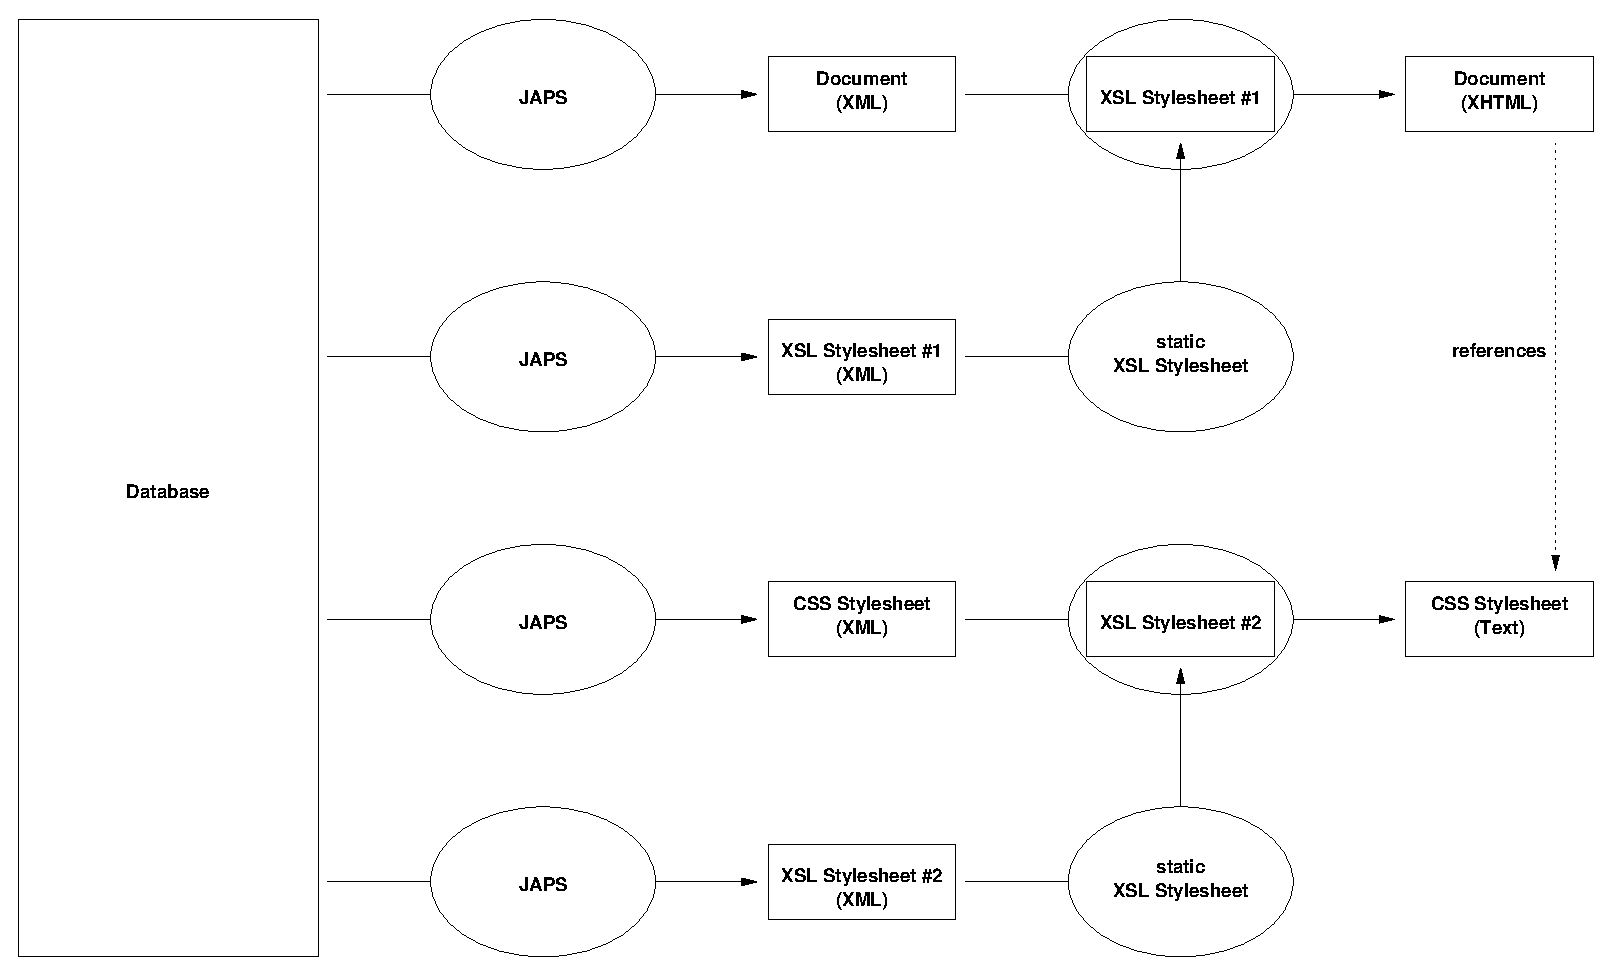
\includegraphics[width=15.5cm]{typical_request_processing.eps}

  \vspace{0.5cm}

  \stepcounter{figure}
  \begin{minipage}{13.5cm}
    \small Figure \thefigure:
    Typical request processing. The resolving of the generic documents is not shown. The
    picture sketches the dynamical creation of an XHTML document, an associated CSS
    stylesheet, and two XSL stylesheets needed to convert the XML of the two
    documents to XHTML and Text/CSS, respectively. The different XSL stylesheets occurring
    in the picture have the following functions: \emph{XSL Stylesheet \#1:} XML-to-XHTML
    conversion; \emph{XSL Stylesheet \#2:} XML-to-Text/CSS conversion; \emph{static XSL
    Stylesheet:} the fixed (not dynamically created) stylesheet converging XML to XSL.
  \end{minipage}
\end{figure}

\end{document}
